\chapter{Preliminary}

As the target platform for this work is the graph database neo4J, we will mostly consider \textit{directed} graphs. From the terminology we always refer \textit{arcs}, which is an directed edge.
In some rare cases we might refer to \textit{edges}. There you can be sure that it doesn't matter weather it is directed or not.

\section{Notation and Expressions}
We denote a graph $G(V, A)$ in case me mean an \textit{directed} graph, where $v$ is a vertex contained in the vertices $v \epsilon  V$ and $e$ is an
edge $a \epsilon A$. An arc is uniquely defined by to vertices $v_a$ and $v_b$ such that $v_a \neq v_b$, so there are no loops nor multi edges.
An edge additionally has a weight function $w: E \rightarrow \mathbb{R}_{<0} $ it's weight which must be a positive.
\\
$G$ represents the input graph. The contraction graph $G'(V', A')$ is the graph that will be used at contraction for initially building the CCH index structure. A vertex $v$ in will 
never be really deleted. Instead the rank property $r(v)$ is set to mark this as an already contracted. So $V \equiv V'$ but $A \subseteq A'$ there will be edges add while building
the CCH index. $S = A' \setminus A$ is the shortcut set that is added throughout the contraction. 
\\
$G^*(V^*, A^*)$ is the is the search graph while doing one a shortest path query. Futhermore one query will have two search graphs. $G^*_\uparrow$ representing the upwards search graph
and the $G^*_\downarrow$.
\\
Finally there will be the edge set of edges that are written to the disk. These will $\bigcirc E$ will be separated into to sets $\bigcirc E_\downarrow$ and $\bigcirc E_\uparrow $, too.


\section{Customizable Contraction Hierarchies}\label{sec:Preliminary_CCH}

In this section we will present the basic idea of \cite[Customization Contraction Hierarchies]{CCH} and also work out the main difference between CCH and \cite[Contraction Hierarchies]{Geisberger_2012}.
It is far form being complete, but there will be some easy examples to show the concept.

\subsection{Contracting and Searching}

\begin{figure}
    \centering
    \input{assets/tikz/contractingAndSeaching.tex}
    \caption{The numbers inside the vertices represent their contraction order}
    \label{fig:contrating_and_searching}
\end{figure}

\subsection{Difference between CH and CCH}

Looking at the left graph in Figure \ref*{fig:DifferenceCHAndCCH} it has been contracted in the CH way, whereas the right is the CCH way. We explicitly state this here because 
we have found paper \cite{Ouyang_2020} that mix up these well known name, claiming they to Contraction Hierarchies while actually doing Customizable Contraction Hierarchies. 
The main difference is, CH will only insert an shortcut between two nodes if the node that is contracted lies on the shortest path between two of its neighbors. In Figure \ref*{fig:DifferenceCHAndCCH} 
the rank and vertex id are the same. When vertex $1$ is contract the is no shortcut inserted as vertex $1$ is not on the shortest path between which is via vertex $4$.
\\
whereas in the CCH case the edge weights do not play a role a contraction time. If a node is contracted and there is no direct connection between two of its neighbors, one has to insert a shortcut. This gives
the advantage that late on we can easily update edge weights without inserting new shortcut, as all possible need shortcut already exist.
\\ 
Let's complete this example by updating the edge $e(2, 4)$ that currently has the weight of $w(e)=1$ to $w(e) = 5$. Now the vertex $1$ is on the shortest path between vertex $2$ and $3$. 
To update the CH graph we have to insert an edge between vertex $2$ and $3$ whereas the popological structure of the CCH remains the same, one only need to update the weight and the middle node of the already give shortcut.

\begin{figure}
    \centering
    \input{assets/tikz/DifferenceCHAndCCH.tex}
    \caption{The left represents a CH and the right a CCH contracted graph}
    \label{fig:DifferenceCHAndCCH}
\end{figure}

\subsection{Metric Dependent Vertex Order}
There are two way to get a suitable vertex order. A so called \textit{metric independent} and a so called \textit{metric dependent} one. The metric independent recursively uses balanced separator to determine a vertex ordering\cite{CCH}. Although this is the superior method, it is not used in this paper writing an algorithm that calculates balanced separators isn't trivial, and we are not aiming for optimizing the contraction process. 
The metric dependent order mainly uses the edge difference $ED$ to determine which vertex is to be contracted next. The $ED$ is determined as the $|edges To Insert| - |edges To Remove|$. The fewer edges are inserted during contraction the fewer edges will be contained by the final graph. However using only the edge differences doesn't lead to desired result. This is because during contraction there will be areas that get less dense than other. There are two problems that can arise. One is that important vertices are not contracted last. The other is the search space of the query gets linear although it could be logarithmic.

\subsubsection{Important Vertices not contracted last}\label{sec:not_contracted_last}

\begin{figure}
    \centering
    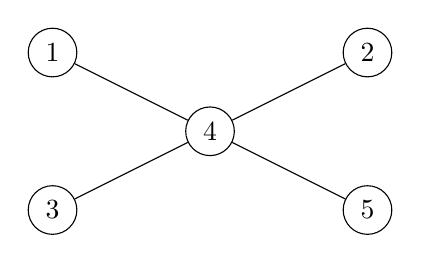
\begin{tikzpicture}[node distance={15mm}, main/.style = {draw, circle}]
    \node[main] (x1) at (1, 2) {$1$}; 
    \node[main] (x3) at (1, 0) {$3$};
    
    \node[main] (x4) at (3, 1) {$4$}; 
    
    \node[main] (x2) at (5, 2) {$2$}; 
    \node[main] (x5) at (5, 0) {$5$}; 
    
    \draw (x1) -- (x4);
    \draw (x2) -- (x4);
    \draw (x3) -- (x4);
    \draw (x5) -- (x4);
    
\end{tikzpicture} 
    
    \caption{The numbers inside the vertices represent their contraction order}
    \label{fig:not_contracted_last}
\end{figure}

Looking at figure \ref{fig:not_contracted_last}, this is a possible contraction order, if only the $ED$ is used to contract vertices. At the beginning the nodes with rank 1, 2, 3, 5 have the same edge difference, which is $ED = -1$. One edge will be removed after contraction and the is no shortcut inserted. This happens until there are only the vertices 4 and 5 left. Now vertex 4 has an $ED=-1$, too, same as vertex 5. Therefore the algorithm contracts the vertex with rank 4 before the one with rank 5. \\
However this is not the desired result. There are six ${(1,2), (1,3), (1,5), (2,3), (2,5), (3,5)}$ shortest paths that involve vertex 4, all the other vertices do not encode any shortest path, so vertex 4 should be contracted last. This can be overcome by the method that is explained in section \ref{sec:vertex_importance}

\subsubsection{Linear Query Search Space}\label{sec:linear_query}

\begin{figure}
\centering
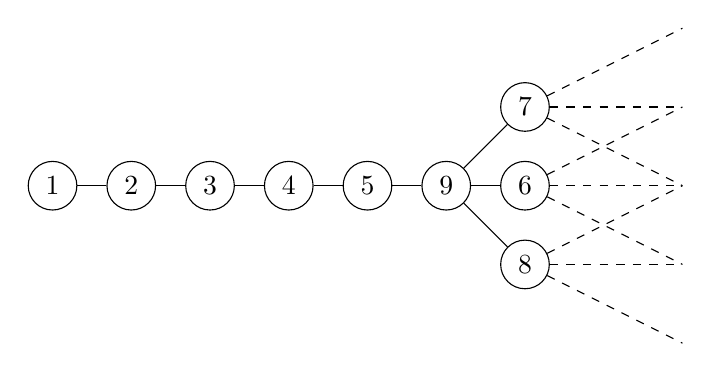
\begin{tikzpicture}[node distance={15mm}, main/.style = {draw, circle}]

    \node[main] (x1) at (0, 0) {$1$};
    \node[main] (x2) at (1, 0) {$2$};
    \node[main] (x3) at (2, 0) {$3$};
    \node[main] (x4) at (3, 0) {$4$};
    \node[main] (x5) at (4, 0) {$5$};
    \node[main] (x9) at (5, 0) {$9$};
    
    \node[main] (x7) at (6, 1) {$7$};
    \node[main] (x8) at (6, -1) {$8$};
    \node[main] (x6) at (6, 0) {$6$};
    
    
    \draw (x1) -- (x2);
    \draw (x2) -- (x3);
    \draw (x3) -- (x4);
    \draw (x4) -- (x5);
    \draw (x5) -- (x9);
    
    \draw (x6) -- (x9);
    \draw (x9) -- (x7);
    \draw (x9) -- (x8);
    
    \draw [dashed] (x7) -- (8, 2);
    \draw [dashed] (x7) -- (8, 1);
    \draw [dashed] (x7) -- (8, 0);
    
    \draw [dashed] (x8) -- (8, 0);
    \draw [dashed] (x8) -- (8, -2);
    \draw [dashed] (x8) -- (8, -1);
    
    \draw [dashed] (x6) -- (8, 1);
    \draw [dashed] (x6) -- (8, 0);
    \draw [dashed] (x6) -- (8, -1);
    
\end{tikzpicture} 
    
\caption{Linear Contraction}
\label{fig:linear_contraction}
\end{figure}

Looking at figure \ref{fig:linear_contraction} this is a possible contraction order using the only the $ED$ as method to determine the importance of a vertex. As you can see vertex 9 is the one with the highest importance. Which is the desire result as all shortest path come from vertices ${1, 2, 3, 4, 5}$ and go any of the vertices ${6, 7, 8}$ have to pass through vertex 9. However regarding only vertices $1, 2, 3, 4, 5$, there is only one way to go when looking for the shortest path. And if we only go left vertex by vertex, there is no difference between our search or a Dijkstra search. Which means, no gain in query performance. Better would be to contract vertex 3 before vertex 2. This would insert one shortcut more which is bearable in sparse areas, but it decreases the hops that need to be done by one as you insert an arc between vertex 2 and 4, so you can surpass vertex 3. 

\subsection{Vertex importance}\label{sec:vertex_importance}

As shown in section \ref{sec:not_contracted_last} and \ref{sec:linear_query} using only the $ED$ as a metric to determine which vertex to contract next is not sufficient to get a suitable

\subsection{Perfect Customization}

\begin{figure}
    \centering
    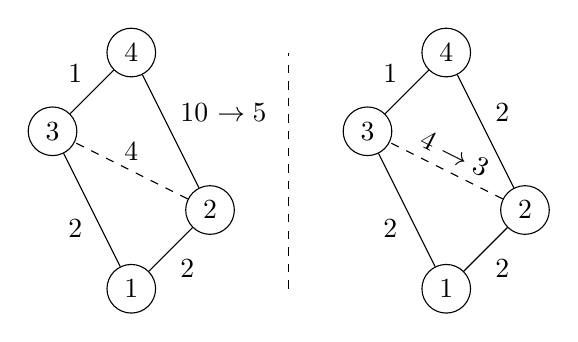
\begin{tikzpicture}[node distance={15mm}, main/.style = {draw, circle}]

    \node[main] (x3) at (0, 2) {$3$};
    \node[main] (x4) at (1, 3) {$4$};
    \node[main] (x2) at (2, 1) {$2$};
    \node[main] (x1) at (1, 0) {$1$};
    
    \draw (x1) -- node[below right] {$2$}(x2);
    \draw (x1) -- node[below left] {$2$} (x3);
    \draw (x2) -- node[above right] {\sout{$10$} $\rightarrow 5$} (x4);
    \draw (x3) -- node[above left] {$1$} (x4);
    \draw[dashed] (x2) -- node[above] {$4$} (x3);

    \draw[dashed]  (3,0) -- (3,3);

    \node[main] (x31) at (4, 2) {$3$};
    \node[main] (x41) at (5, 3) {$4$};
    \node[main] (x21) at (6, 1) {$2$};
    \node[main] (x11) at (5, 0) {$1$};
    
    \draw (x11) -- node[below right] {$2$}(x21);
    \draw (x11) -- node[below left] {$2$} (x31);
    \draw (x21) -- node[above right] {$2$} (x41);
    \draw (x31) -- node[above left] {$1$} (x41);
    \draw[dashed] (x21) -- node[above, sloped] {\sout{$4$} $\rightarrow 3$}  (x31);

    
\end{tikzpicture}
    \caption{Disk Block}
    \label{fig:perfectCustomization}
\end{figure}

Here is an example why perfect customization is necessary to get the full
benefit of CCH.


